% !TEX root = ../master.tex
\chapter{Implementation and Evaluation}
\label{chap:impl}

In this chapter the implementation of the two artifacts identified and designed in the previous chapter is executed.
First, an attempt is made to implement the visual volume detection system and test it out in a real-world test environment.
Then simulation of an elevator system is implemented to compare tree scheduling strategies and the results of this simulation are evaluated.


\section{Visual System}
TODO
\subsection{Implementation with OpenCV and Python}



based on \autocite[][]{xocoatzin2013voxelcarving}

follows approach up to volume reconstruction, which however is done orthographically

TODO Dependencies:
\begin{itemize}[noitemsep]
    \item \texttt{numpy}:  Provides typed n-dimensional arrays to store image data
    \item \texttt{scipy}:  Dependency of scikit-image
    \item \texttt{matplotlib}: Used for plotting of 2D graphs
    \item \texttt{opencv-python}: Open Computer Vision library
    \item \texttt{opencv-contrib-python}: Provides additional functions for OpenCV
    \item \texttt{PyYAML}: Used for parsing and writing of \ac{YAML} files in the camera calibration
    \item \texttt{scikit-image}: Image processing functions  
    \item \texttt{PyQt5}: Dependency of \texttt{pyqtgraph}, used to create application windows
    \item \texttt{PyOpenGL}: Dependency of \texttt{pyqtgraph}, used for for \ac{3D} rendering 
    \item \texttt{pyqtgraph}: Used to display real-time 3D graphs
\end{itemize}

TODO
\subsection{Test Execution}
elevator setup: measurements, camera positions
scenario: empty, single person, 2 persons, 3 persons, only carton, 1+ carton, 2+ carton
TODO

\begin{figure}[p]
    \centering
    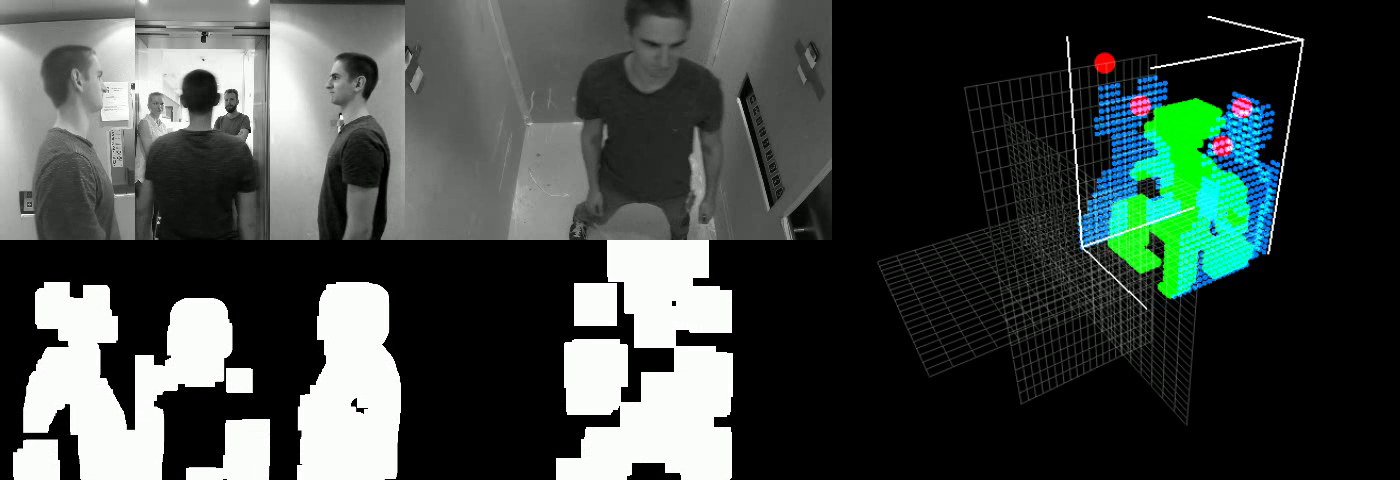
\includegraphics[width=1.0\textwidth, keepaspectratio]{volumeintersection_preview_04}
    
    \vspace{0.5em}
    
    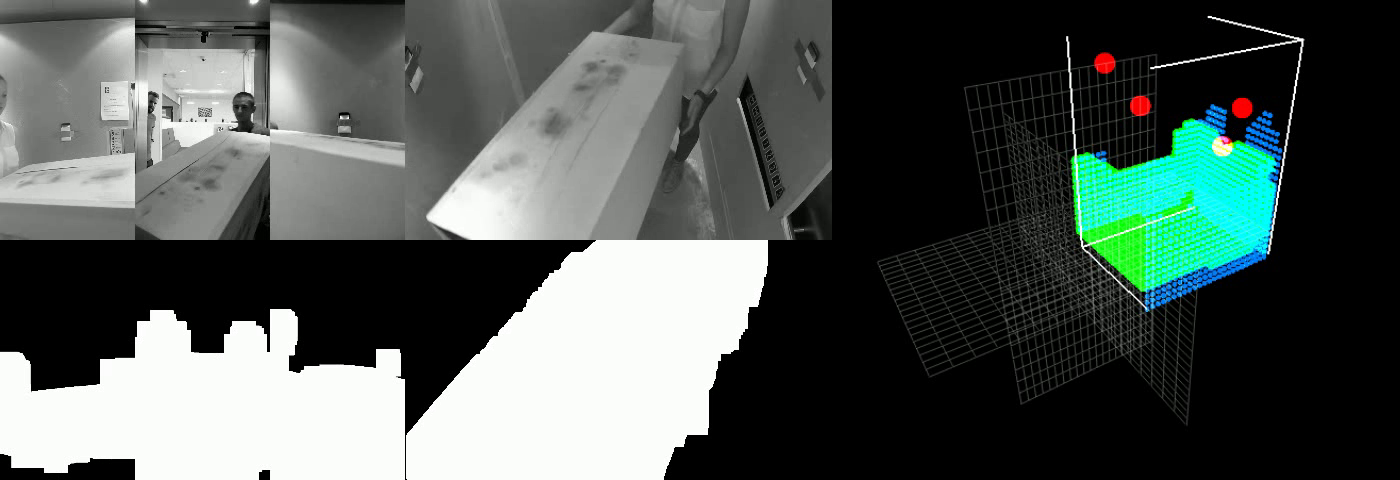
\includegraphics[width=1.0\textwidth, keepaspectratio]{volumeintersection_preview_03}
    
    \vspace{0.5em}
    
    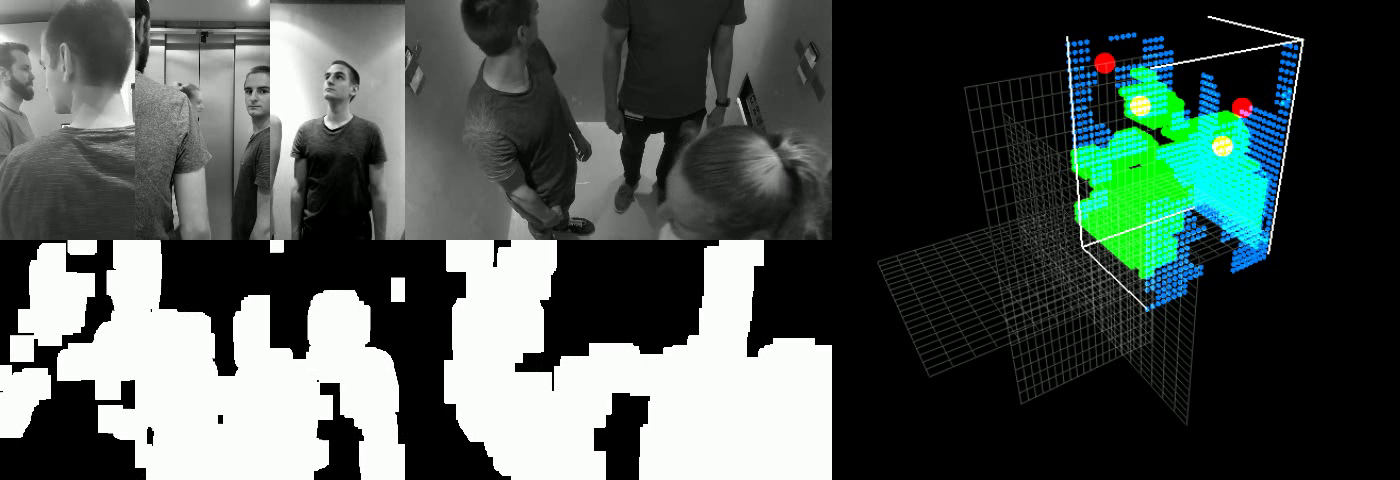
\includegraphics[width=1.0\textwidth, keepaspectratio]{volumeintersection_preview_05}
    
    \caption[Images of volume intersection test with orthogonal projection]{Images of volume intersection test with orthogonal projection. Each preview showing the camera images, foreground masks and the resulting volume intersection. (a) single passenger (b) cargo object (c) multiple passengers.}
    \label{fig:impl:preview}
\end{figure}

\subsection{Result Evaluation}
general concept feasible
small viewing angle: person out of frame
poor foreground separation by only applying background subtraction
non-correct othorgonal intersection implemented

TODO

\section{Scheduling Algorithm}
TODO
\subsection{Implementation of Simulation}

The simulation is implemented in the \emph{Rust} programming language.
Rust is a programming language initially developed by Mozilla.
According to its website it is a \enquote{systems programming language that runs blazingly fast, prevents segfaults, and guarantees thread safety} \autocite{rust2018rust}.
It features an expressive static type system and can be used to build applications that take advantage of modern hardware
\autocite[][]{matsakis2014rust}.
The rust compiler targets common platforms and operating and compiles source code to native machine code.
The language is chosen, since the author is proficient in it.

TODO überleitung

TODO

The \texttt{main} function is the entry point into the program.
In it the general behavior of the simulation is defined.
It initializes the simulation parameters and traffic patterns and runs the actual simulation runs.
The actions it performs can be described as following:
\begin{enumerate}
    \item Initialize the \texttt{BuildingParameters b}, \texttt{LiftParameters l} and\\ \texttt{SimulationParameters s}.
    \item Generate \texttt{s.simulations} many traffic \texttt{TrafficGenerator} instances, which each generates a traffic pattern. A traffic patterns describes the arrivals of traffic items for each tick of the simulation period. A Poisson distribution can be used to determine the amount of traffic items that arrive within this tick \autocite{beers2015arrivals}.
    \item For each traffic patterns, run the simulation with the three different scheduling strategies. Each simulation is given the same parameters (\texttt{b, l, s}) and the same traffic pattern. The procedure to run a single simulation is described below.
    \item Collect the results of all simulations and filter out the results of any run, where any of the three strategies produced an invalid result.
    \item Calculate the specified metrics by aggregating all the results for each strategy.
\end{enumerate}


The actions takes in order to run a single simulation are then as follows:
\begin{enumerate}
    \item Create a new \texttt{ElevatorSystem e}, which holds the system state to be altered during the simulation.
    \item Create an empty \texttt{SimulationResults} metric container, which will aggregate the metrics for this run.
    \item While \texttt{e.ticks < s.total\_ticks()}, repeat the following simulation cycle:
    \begin{enumerate}
        \item Ask the control strategy for an action to be performed on the elevator system based on the current state of said system and the internal state of the control strategy.
        The action can be one of the actions listed as \texttt{ControlAction}.
        \item Perform the given action on the elevator system, thereby updating all fields effected by this action.
        \item Calculate the time it took to perform those action on the system and advance the ticks accordingly.
        \item Update the  metrics about waiting and ride time for each traffic item that is currently in the floor queues or in the elevator. Also update the metrics about the number of delivered traffic items and elevator stops.
        \item Copy the traffic item form the traffic pattern into the floor queues, which arrived in the time between the last tick and the updated tick.
    \end{enumerate}
    \item Correct the gathered metrics by removing the ride times of traffic items, who did not arrive at their destination yet and waiting times of traffic items, who did not yet enter the elevator.
\end{enumerate}

TODO reference implementation of the strategies

The three control strategies are passed to the execution of a single simulation as generic parameters parameters.
Therefore, they all implement an interface \texttt{ControlStrategy}.
The control strategies decide in each tick of the simulation, which action should be taken on the elevator system


TODO reference and describe class diagram in figure \ref{fig:impl:simclass}
rust does not support only the oop style, so a class diagram is not compleatly suitable

\begin{figure}[p]
    \centering
    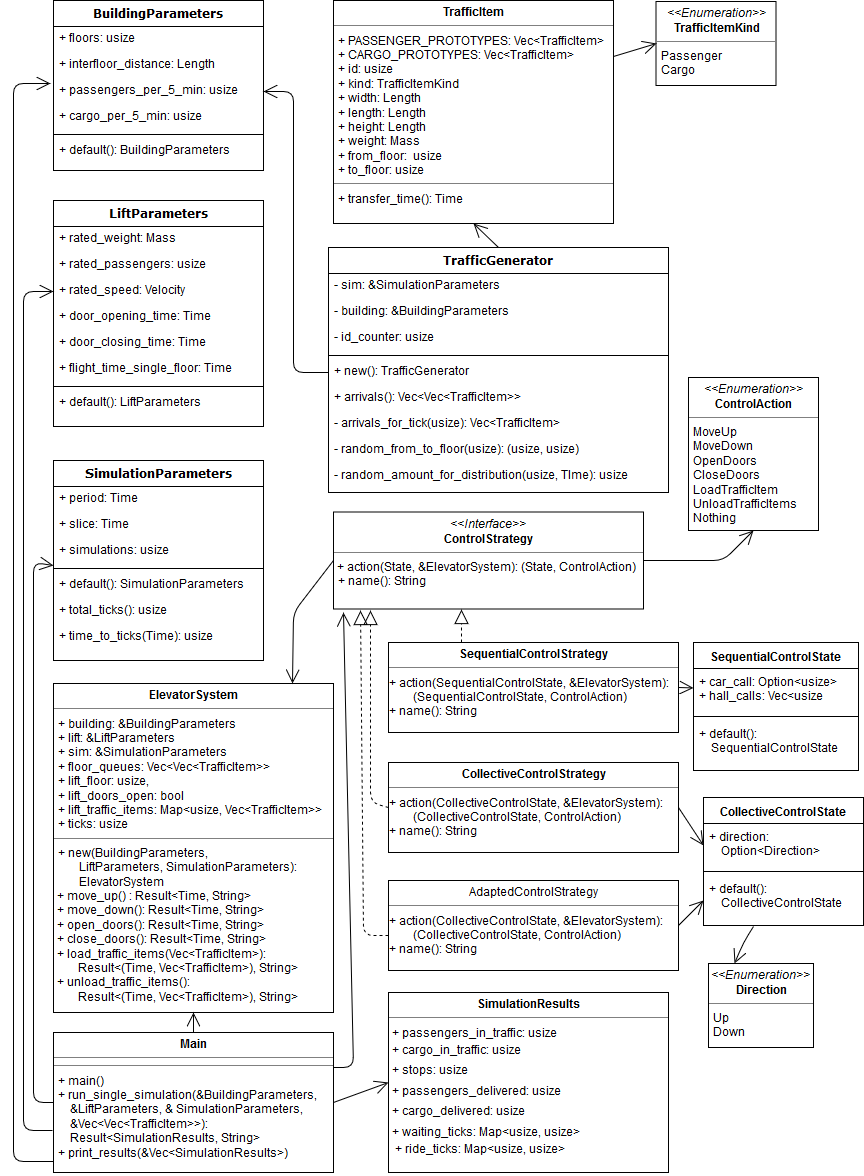
\includegraphics[width=1.0\textwidth, keepaspectratio]{sim_uml_class}
    \caption{Class diagram for the elevator simulation program}
    \label{fig:impl:simclass}
\end{figure}

TODO dependecies:
\begin{itemize}[noitemsep]
    \item \texttt{lazy\_static}: Used for initialization of prototype list
    \item \texttt{rand}: Provides randomness functions and common likelihood functions including the Poisson distribution
    \item \texttt{rayon}: Provides data-driven multi-threading capabilities and is used to run the simulations in parallel
    \item \texttt{streaming-stats} (\texttt{stats}): Provides functions to create metrics with online algorithms such as average,  minimum, maximum and standert deviation
    \item \texttt{uom}: Provides types for units of measurements such as Mass and Time, as well as the respective \ac{SI} units such as kilograms and seconds
\end{itemize}


\subsection{Evaluation of Simulation Results}

\begingroup
\renewcommand*{\arraystretch}{1.0}
\begin{table}[]
\centering
\begin{tabular}{llrrr}
                                      &     & \begin{minipage}{2cm}\textbf{Sequential Control} \vspace{1em}\end{minipage} & \begin{minipage}{2cm}\textbf{Collective Control} \vspace{1em}\end{minipage} & \begin{minipage}{2cm}\textbf{Adaptive Control} \vspace{1em}\end{minipage}\\ \hline
\multirow{4}{*}{\textbf{Total passengers}}     & \textbf{min}        & 57.00                                                                                                                                             & 57.00                                                                                                                                             & 57.00                                                                                                                                           \\
                                               & \textbf{max}        & 113.00                                                                                                                                            & 113.00                                                                                                                                            & 113.00                                                                                                                                          \\
                                               & \textbf{avg}        & 84.09                                                                                                                                             & 84.09                                                                                                                                             & 84.09                                                                                                                                           \\
                                               & \textbf{$ \sigma $} & 8.97                                                                                                                                              & 8.97                                                                                                                                              & 8.97                                                                                                                                            \\ \hline
\multirow{4}{*}{\textbf{Total cargo}}          & \textbf{min}        & 9.00                                                                                                                                              & 9.00                                                                                                                                              & 9.00                                                                                                                                            \\
                                               & \textbf{max}        & 42.00                                                                                                                                             & 42.00                                                                                                                                             & 42.00                                                                                                                                           \\
                                               & \textbf{avg}        & 24.10                                                                                                                                             & 24.10                                                                                                                                             & 24.10                                                                                                                                           \\
                                               & \textbf{$ \sigma $} & 4.95                                                                                                                                              & 4.95                                                                                                                                              & 4.95                                                                                                                                            \\ \hline
\multirow{4}{*}{\textbf{Stops}}                & \textbf{min}        & 102.00                                                                                                                                            & 93.00                                                                                                                                             & 96.00                                                                                                                                           \\
                                               & \textbf{max}        & 135.00                                                                                                                                            & 158.00                                                                                                                                            & 157.00                                                                                                                                          \\
                                               & \textbf{avg}        & 118.47                                                                                                                                            & 125.75                                                                                                                                            & 129.60                                                                                                                                          \\
                                               & \textbf{$ \sigma $} & 5.22                                                                                                                                              & 10.41                                                                                                                                             & 9.30                                                                                                                                            \\ \hline
\multirow{4}{*}{\textbf{Passengers delivered}} & \textbf{min}        & 37.00                                                                                                                                             & 46.00                                                                                                                                             & 53.00                                                                                                                                           \\
                                               & \textbf{max}        & 65.00                                                                                                                                             & 107.00                                                                                                                                            & 108.00                                                                                                                                          \\
                                               & \textbf{avg}        & 49.32                                                                                                                                             & 78.06                                                                                                                                             & 79.67                                                                                                                                           \\
                                               & \textbf{$ \sigma $} & 4.24                                                                                                                                              & 9.45                                                                                                                                              & 8.75                                                                                                                                            \\ \hline
\multirow{4}{*}{\textbf{Cargo delivered}}      & \textbf{min}        & 3.00                                                                                                                                              & 3.00                                                                                                                                              & 4.00                                                                                                                                            \\
                                               & \textbf{max}        & 23.00                                                                                                                                             & 29.00                                                                                                                                             & 33.00                                                                                                                                           \\
                                               & \textbf{avg}        & 14.13                                                                                                                                             & 14.61                                                                                                                                             & 19.80                                                                                                                                           \\
                                               & \textbf{$ \sigma $} & 3.20                                                                                                                                              & 3.54                                                                                                                                              & 4.38                                                                                                                                            \\ \hline
\multirow{4}{*}{\textbf{Waiting time / s}}     & \textbf{min}        & 1.50                                                                                                                                              & 0.00                                                                                                                                              & 0.00                                                                                                                                            \\
                                               & \textbf{max}        & 2873.50                                                                                                                                           & 202.60                                                                                                                                            & 662.70                                                                                                                                          \\
                                               & \textbf{avg}        & 688.09                                                                                                                                            & 41.25                                                                                                                                             & 53.03                                                                                                                                           \\
                                               & \textbf{$ \sigma $} & 499.11                                                                                                                                            & 32.63                                                                                                                                             & 48.98                                                                                                                                           \\ \hline
\multirow{4}{*}{\textbf{Ride time / s}}        & \textbf{min}        & 13.00                                                                                                                                             & 13.00                                                                                                                                             & 13.00                                                                                                                                           \\
                                               & \textbf{max}        & 64.00                                                                                                                                             & 2180.20                                                                                                                                           & 1809.70                                                                                                                                         \\
                                               & \textbf{avg}        & 29.57                                                                                                                                             & 125.35                                                                                                                                            & 102.29                                                                                                                                          \\
                                               & \textbf{$ \sigma $} & 13.92                                                                                                                                             & 160.37                                                                                                                                            & 130.77                                                                                                                                         
\end{tabular}
\caption{\label{tab:impl:simulationresults} Simulation results for tested scheduling algorithms}
\end{table}
\endgroup

By running the  implemented simulation, the results displayed in table \ref{tab:impl:simulationresults} are gathered.
It is visible, that the three scheduling algorithms have distinct manifestations of the metrics that are recorded.
The sequential control sets focus on low ride time, the collective control sets focus on a balance between wait and ride time while maintaining a high delivery rate. 
The adaptive control strategy favours the delivery of cargo objects with lower ride times, while trading for a higher waiting time.
The key takeaways, expressed in relative numbers, here are:

\begin{itemize}
    \item Adaptive control delivers \textbf{more cargo items} on average than sequential control (\texttt{+}40.13~\%) and collective control (\texttt{+}35.52~\%).
    \item Collective control (\texttt{+}58.27~\%) and adaptive control (\texttt{+}61.53~\%) deliver \textbf{more passengers} on average compared to sequential control. 
    \item Sequential control shows a drastically higher mean waiting time then the other two (\texttt{+}1568.09~\%, \texttt{+}1297.55~\%). However, it features a lower average ride time (\texttt{-}76.41~\%, \texttt{-}71.09~\%), which is is only linear dependent on the travel distance.
    \item Adaptive control shows a slightly higher average waiting time (\texttt{+}30.56~\%) but has a lower (\texttt{-}18.40~\%) average ride time, which is less spread (\texttt{-}18.46~\%) compared to collective control.
\end{itemize}

In conclusion these results for the adaptive control show, that giving cargo items priority and delivering them in a sequential style, while delivering passengers in a collective style, 
can increase the amount of cargo that gets delivered. 
This reduces the average ride time, however it comes with a trade-of in waiting time.
The increased performance can be explained by the reduced time, the cargo items block the space and weight restrictions present in the elevator cabin and prevent other passengers from entering.
Therefore delivering them faster causes a shorter blocking of theses resources, resulting in a better overall utilization.

The precondition of applying the adaptive control strategy is the knowledge, 
whether a cargo objects is currently inside the elevator cabin and is blocking it for other passengers 
and the information about the destination of this object.
This information can be obtained by combining the visual system presented before, which is capable of detecting cargo objects by their volume, with the information about car calls made for this object. To create the association of an object present in the lift and its destination, 
the time of entering the cabin and performing the car call can be correlated.
Otherwise, in an environment that features hall calls with information about the destination, this association can be used.
An alternative would be an \emph{override} button in the cabin, 
to give priority to the current car call, regardless of the presence of an cargo object in the cabin.

However the scenario chosen for the simulation is very specific and can benefit from the kinds of optimizations the adaptive control yields. 
The given traffic conditions in a multi-story building with a single elevator, 
which is used by passengers and cargo alike, 
do favour the prioritization of cargo items by sequentially delivering them.
The results for other traffic patterns, e.g. for elevators that only convey passengers,
might differ and might not benefit from an adapted scheduling.

\section{Economic Considerations}
As stated above, the presented scheduling algorithm can use the visual system to determine the presence of a cargo object, which can benefit the handling capacity of elevators which are regularly used by passengers and cargo items.
There are several possible real-life scenarios with these properties:
\begin{itemize}
    \item \textbf{Hospitals} with elevators where patient beds are moved. The medical beds are usually as large as the elevator allows and therefore block the elevator from being used by groups of additional passengers. Additionally, patients with medical conditions who occupy the bed often should have a prioritized transport, as their health might depend on every second spent in the elevator. 
    \item Large office buildings with \textbf{auxiliary lifts} that are used by janitors and craftsman, who carry carts, tool cabinets or hardware material. These lifts could also be used by regular passengers and might even be integrated into an elevator group. However, the cart could block the elevator.
    \item Multi-storey \textbf{Warehouses} or \textbf{fabrication plants} with heavy duty cargo lifts used 
    by factory employees and forklifts or other transportation devices for heavy goods. The lifts block each other from entering the lift and therefore need to be handled sequentially. 
\end{itemize}

Possible customers for DXC Technology and the Digital Service Innovation team are Otis, Kone, Schindler and Thyssen, which \textcite[][p.~4]{unger2015aufzuege} identifies as the biggest elevator companies. Some of those companies already have business relations with DXC Technology and therefore might be interested in setting up an innovative project to explore the ideas presented in this paper.
They could consider offering an elevator system with an integrated visual system to customers with the needs described above, who construct a new building or want to upgrade an existing lift, as an optional feature at an additional charge.

The cost structure for the visual solution is threefold. 
A project implementing this or a similar solution generates cost during development, installation of the individual solution and later operation.
Since elevator technology experts and computer vision experts need to work together for the development of an advanced visual solution in elevators, 
the costs in this phase are characterized by expenses for said experts, as well as laboratory equipment.
Developing resilient and high-quality software requires careful planning and implementation and is therefore crucial for the costs at this stage.
When installing the  solution into an elevator cabin and integrating it into the control circuit, the costs are governed by the hardware installed and the labor of the technician installing it. 
The costs for the hardware includes multiple cameras, do neither need an extraordinary high resolution nor frame rate, and a general purpose computer to process the images, which needs to have enough computing power to process the images in near real-time. 
Furthermore, a connection to the elevator controller is necessary which might require some kind of adapter.
During operation, the costs are reduced down to the electricity consumed by the additional components and  the costs for maintaining the system.

Possible savings from implementing the proposed visual system and the scheduling algorithm manifest in the faster delivery of cargo items and therefore the reduction of the time they block the cabin for other passengers. 
This can result in a higher overall passenger throughput and therefore reduce the energy needs per passenger.
Furthermore, the faster delivery of cargo objects can have impacts on the costs associated with their travel time, which highly depend on the type of good that is transported and the environment it is situated in. 
For example in a production plant, reduced transport times for the produced goods could lead to reduced production costs in general.


\section{Privacy Considerations}
Installing a camera system unavoidably raises privacy and security concerns 
for the filmed individuals.
Especially in elevators, which are publicly accessible, there are legal requirements to fulfill.
In Germany the Federal Data Protection Act, \\
\ac{BDSG} \autocite[][]{bmjv2009bdsg}, 
regulates the usage of video surveillance systems.
Public areas may only be observed for specified purposes.
The presence of a surveillance system must be indicated,
as well as the name and contact of its controller. 
When the data gathered by the system is no longer needed for the specified purpose, it must be deleted 
\autocite[][§~4]{bmjv2009bdsg}.
The European \ac{GDPR} \autocite{eu2016gdpr} describes similar, more broad principles:  
\emph{data transparency, purpose limitation, data minimization, storage limitation and confidentiality}
\autocite{ico2018gdpr}.
Oriented at this principle the following paragraphs provide privacy consideration about the visual system.

The presented visual system has a \emph{limited purpose}, in that it is only used 
to determine whether passengers or cargo items are present in the elevator cabin 
and what volume they take up. 
This information is used to improve the scheduling of the elevator.

In order to keep the usage of video data \emph{transparent},
passengers should be informed about the video system before they enter the cabin.
This could be done by installing a sign, which indicates the presence of the video system, 
clearly states, for what purpose the video data is used for, 
and who is operating the system and can be contacted in case of issues.
The sign should be in front and inside of the elevator, 
so that potential passengers can decide,
if they want to use the lift and be filmed.

Since the system has a limited purpose, 
only data specific to that purpose should be gathered and processed.
The data usage should be \emph{minimized}.
Only as few cameras as possible, but as many as necessary should be installed in the lift.
Areas that are not of interest for the lift system should not be filmed.
Furthermore, the resolution of the cameras should be only as high as necessary.
For purpose of detecting the presence, position, and outline of a passenger or cargo object 
in the cabin, it is not required to capture fine details.
The DIN EN 62676-4 norm \autocite[][]{din2016surveillance} recommends 
to use a camera resolution, which captures 25 to 62.5 pixel per meter,
for the purpose of detecting or monitoring people.
In addition, the kind of processing of the video data should be limited to the extent necessary for the purpose of the video system. 
For example, it is not necessary to perform face detection  or to identify individuals.
However, tracking the path of an individual over the course of their journey might be beneficial for the application.

The presented system can operate in real time.
Only the current video frame is needed to determine the presence and volume of passengers and objects.
Therefore, the \emph{storage} of the video data can be \emph{limited}.
There is no need to store the video data at all.

In order to keep the video data \emph{confidential}, 
measures must be taken to prevent access by unauthorized parties.
For the purpose of the system, all data processing can be done locally within the elevator system.
The visual system only needs to interact with the elevator controller.
Therefore there is no need to make the data available to the outside, e.g. the internet.
Doing so would open up unnecessary possibilities for misuse of the video system.
